\begin{figure*}[p]
\centering
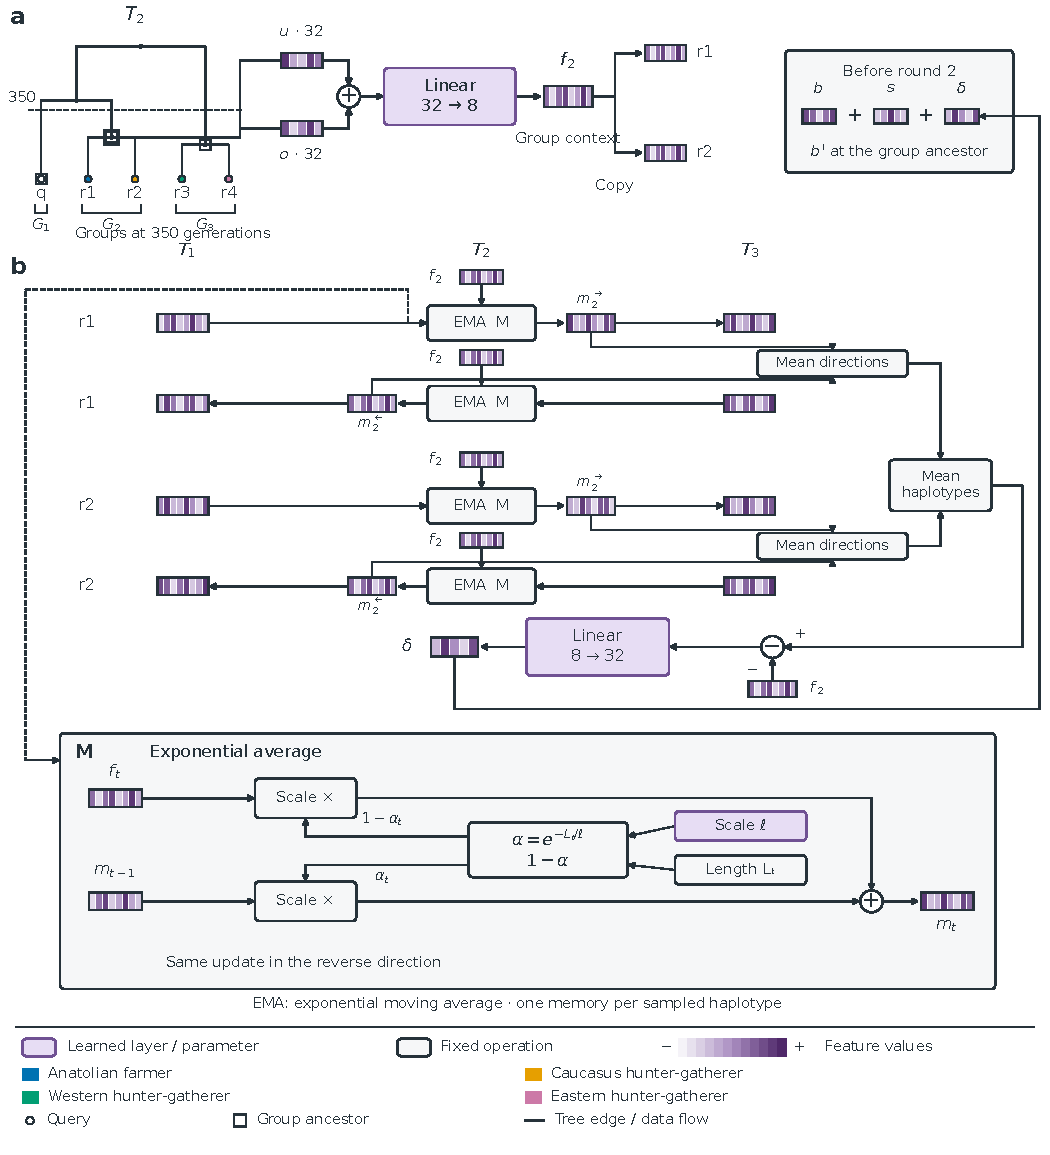
\includegraphics[width=\textwidth]{figures/TreeLoom_memory.pdf}
\caption{\textbf{a,} The age cut produces groups $G_1,G_2,G_3$. The marked ancestor of r1 and r2 supplies upward and outside states. Their sum projects to $f_2$, copied to both group members. The complete tree remains in the GNN.
\textbf{b,} Each haplotype retains separate forward and reverse exponential memories. Both labeled $m_2$ outputs are states at $T_2$. Direction means are computed per haplotype, then averaged within the current group. Subtracting $f_2$ and projecting gives correction $\delta$, added at the group ancestor before round 2. The connected expansion of M shows both vector and scalar inputs. Interval length $L_t$ and learned scale $\ell$ determine retention $\alpha_t$. The first state in each direction equals its current context. The same update applies at other intervals, whose context inputs are omitted. This exponential memory is distinct from the final BiGRU. Feature values are illustrative.}
\label{fig:memory}
\end{figure*}
